
\begin{frame}{The basic problem}

%\adjincludegraphics[width=0.9\textwidth,trim={0 {.5\height} 0 0 }, clip]{static_figures/survey_and_voting.jpg}

We have a survey population, for whom we observe:
%
\begin{itemize}
 \item Covariates $\x$ (e.g.~race, gender, zip code, age, education level)
 \item Responses $\y$ (e.g.~A binary response to ``do you support candidate Z'')
\end{itemize}
%

We want the average response in a target population,
in which we observe only covariates.


\splitpage{
    \centering
    \only<1>{
    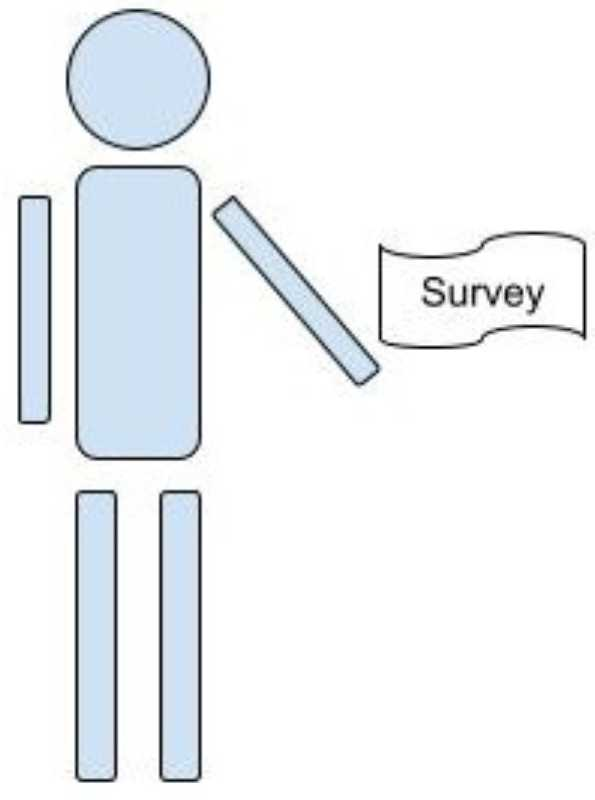
\includegraphics[width=0.5\textwidth]{static_figures/survey_man.jpg}
    }
    \only<2->{
    %
\includegraphics[width=0.5\textwidth]{static_figures/survey_crazy_man.jpg}
    
\includegraphics[width=0.5\textwidth]{static_figures/guinea_pig.png}
    }
}{
    \centering
    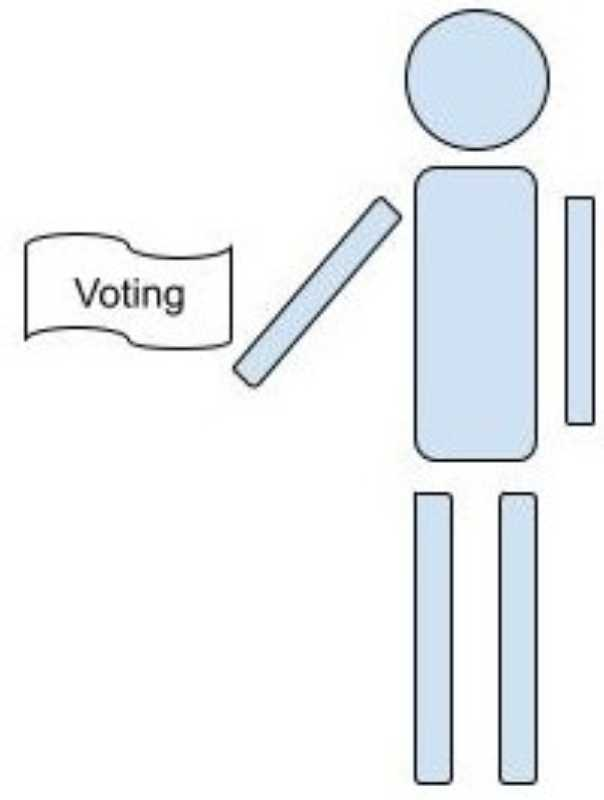
\includegraphics[width=0.5\textwidth]{static_figures/voting_man.jpg}
}

\splitpage{
    \centering
    Observe \surcol{$(\x_i, y_i)$ for $i = 1, \ldots, \nsur$}\\
}{
    \centering
    Observe \tarcol{$\x_j$ for $j = 1, \ldots, \ntar$}\\
}

\onslide<2->{
\textbf{The problem is that the populations may be very different, maybe leading to bias.}
\footnote{Photo copyright: Mark Taylor / \texttt{naturepl.com}}
}

\onslide<3->{
    How can we use the covariates
    to say something about the target responses?
}
%
\end{frame}

%%%%%%%%%%%%%%%%%%%%%%%%%%%%%%%%%%%%%%%%%%%%%%%%%%%%%%%
%%%%%%%%%%%%%%%%%%%%%%%%%%%%%%%%%%%%%%%%%%%%%%%%%%%%%%%
%%%%%%%%%%%%%%%%%%%%%%%%%%%%%%%%%%%%%%%%%%%%%%%%%%%%%%%

\begin{frame}[t]{Two approaches}

We want $\tarcol{\mu := \meantar \y_j}$,
but don't observe target $\tarcol{\y_j}$.  Let $\surcol{\Ysur = \{\y_1, \ldots, \y_{\Nsur}\}}$.

\begin{itemize}
    \item Assume $p(y | \x)$ is the same in both populations,
    \item But the distribution of $\x$ may be different in the survey and target.
\end{itemize}
%
\pause

\splitpagenoline{
    \centering
    \textbf{Calibration weighting}
}{
    \centering
    %\textbf{Multilevel regression and poststratification (MrP)}
    \textbf{Bayesian hierarchical modeling (MrP)}
}
%
%\\\hrulefill\\
\\[1em]
%
\splitpagenoline{
    \centering
    $\blacktriangleright$
    Choose ``calibration weights'' \surcol{$w_i$}\\
    using only the regressors $\x$\\
    (e.g.~raking weights)
}{
    \centering
    $\blacktriangleright$
    Choose $\expect{}{\y \vert \x, \theta} = m(\theta^\trans \x)$,\\
    choose prior $\p(\theta | \Sigma) \p(\Sigma)$\\
    (e.g.~Hierarchical logistic regression)
} \pause
%
\\[1em]
\splitpagenoline{
    \centering
    $\blacktriangleright$ Take
    $\muhatcw = \surcol{\meansur w_i y_i}$
}{
    \centering
    $\blacktriangleright$ Take
    $\tarcol{\yhat_j} =
        \expect{\postsur}{\y | \tarcol{\x_j}}$ and\\
    $\muhatmrp = \tarcol{\meantar \yhat_j}$
}\pause
%
\\[1em]
\splitpagenoline{
    \centering
    $\blacktriangleright$ Dependence %of \surcol{$\muhat_{\cal}$}
    on \surcol{$\y_i$} is clear\\
    % (\surcol{$\w_i$} typically chosen using only $\x$)
}{
    \centering
    $\blacktriangleright$ Dependence %of \surcol{$\muhat_\mrp$}
    on \surcol{$\y_i$} very complicated\\
    (Typically via MCMC draws from $\postsur$)
}\pause
%
\\[1em]
\splitpagenoline{
    \centering
    $\blacktriangleright$ Weights give interpretable diagnostics:
    %
    \begin{itemize}
        \item Frequentist variability
        \item Regressor balance
        \item Partial pooling
        %\item Extrapolation
    \end{itemize}
    %
}{
    \centering
    $\blacktriangleright$ \textbf{Black box}\\
    \pause
    \vspace{1em}
    $\leftarrow$ Today, we'll open the box and provide
        MrP analogues of all these diagnostics
}


\end{frame}


%%%%%%%%%%%%%%%%%%%%%%%%%%%%%%%%%%%%%%%%%%%%%%%%%%%%%%%
%%%%%%%%%%%%%%%%%%%%%%%%%%%%%%%%%%%%%%%%%%%%%%%%%%%%%%%
%%%%%%%%%%%%%%%%%%%%%%%%%%%%%%%%%%%%%%%%%%%%%%%%%%%%%%%

\begin{frame}[t]{Prior work: Equivalent weights for linear models}

\splitpagenoline{
\centering
Calibration weighting estimators:\\[1em]
$\muhatcw = \surcol{\meansur w_i y_i}$.}{
\centering
MrP estimators:\\[1em]
$\muhatmrp = \tarcol{\meantar \yhat_j}$
}

\onslide<2->{
\vspace{1em}
\textbf{...sometimes coincide!}\\[1em]
\textcite{gelman:2007:struggles} observes that MrP is a weighting estimator when
$\yhat$ is computed with OLS:
$$
\begin{aligned}
\muhatmrp ={}& \tarcol{\meantar \yhat_j} =
\tarcol{\meantar }
\underbrace{\tarcol{\x_j^\trans} \surcol{\betahat}}_{\textrm{Linear in }\surcol{\Ysur}} =
\surcol{\meansur} \surcol{\w_i^{\ols} \y_i}
\end{aligned}
$$
}

\only<3>{
Most existing literature on comparing weighting and MrP focus on such linear models.
\footnote{
    For example,
    \textcite{gelman:2007:struggles,benmichael:2021:multilevel,chattopadhyay:2023:implied}.}


But what if you use a non--linear link function?  Or a hierarchical model?\\
\vspace{2em}
\hrulefill
\begin{displayquote}
``It would also be desirable to use nonlinear methods  ...
but then it would seem difficult to construct
even approximately equivalent weights.  Weighting and fully nonlinear models
would seem to be completely incompatible methods.''
--- \parencite{gelman:2007:strugglesrejoinder}
\end{displayquote}
\vspace{1em}
}


\only<4>{
\textbf{Useful note.}  We know the OLS formula, so we can write out $\surcol{\w_i^{\ols}}$ by hand.\\[1em]
But we only had access to $\muhatmrp$ as a black box, we could compute
$$
\surcol{\w_i^{\ols}} = \nsur \frac{\partial \muhatmrp}{\partial \surcol{\y_i}}.
$$
}

\end{frame}






%%%%%%%%%%%%%%%%%%%%%%%%%%%%%%%%%%%%%%%%%%%%%%%%%%%%%%%
%%%%%%%%%%%%%%%%%%%%%%%%%%%%%%%%%%%%%%%%%%%%%%%%%%%%%%%
%%%%%%%%%%%%%%%%%%%%%%%%%%%%%%%%%%%%%%%%%%%%%%%%%%%%%%%

\begin{frame}[t]{Logistic regression is generally nonlinear}

\def\alphav{\mathbf{\alpha}}
%
\begin{itemize}
    \item Suppose the model is $\m(\x^\trans \theta) = \mathrm{Logistic}(\x^\trans \theta)$, with MLE $\thetahat$.
%    \item MrP is $\muhatmrp = \tarcol{\meantar \m(\x_j^\trans \thetahat)}$.
\end{itemize}

The map from $\surcol{\Ysur} \mapsto \tarcol{\m(\x_j^\trans \thetahat(\surcol{\Ysur}))}$ is
\emph{typically globally nonlinear}.

\onslide<2->{
\textbf{Example:} $x_i \sim \mathrm{Unif}[-0.5, 0.5]$, $\y_i \iid \mathrm{Binomial}(1/2)$.
%
Let $\ytil_i(\delta) = \y_i + \delta \ind{x_i > 0.2}$.

The path $\surcol{\delta \mapsto \Ysur(\delta)}$ is well-defined even when $\y$ is supposed to be binary!
}

\only<3>{
Many estimators are also well-defined for small enough $\delta$ under mild conditions.\\

(E.g., OLS, logistic regression MLE, Bayesian posterior.)

% $\Rightarrow$ Each $\delta$ gives a different OLS fit $\betahat(\delta)$ and logistic regression coefficient $\thetahat(\delta)$.

% $\Rightarrow$ Each $\delta$ gives a different prediction $\yhat(\delta)$ at a given $\x$.
}


\only<4>{
For OLS, $\delta \mapsto \tarcol{\betahat(\delta) x}$ is linear.
%
For logistic regression $\delta \mapsto \tarcol{m(\thetahat(\delta) x_j)}$ is non-linear.
\wholeslidefig{
\SimulationPlot{}
}
}

\end{frame}


%%%%%%%%%%%%%%%%%%%%%%%%%%%%%%%%%%%%%%%%%%%%%%%%%%%%%%%
%%%%%%%%%%%%%%%%%%%%%%%%%%%%%%%%%%%%%%%%%%%%%%%%%%%%%%%
%%%%%%%%%%%%%%%%%%%%%%%%%%%%%%%%%%%%%%%%%%%%%%%%%%%%%%%

\begin{frame}[t]{Local weights for nonlinear hierarchical logistic regression MrP}
%
\vspace{-1em}
\begin{itemize}
    \item Suppose the model is $\m(\x^\trans \theta) = \mathrm{Logistic}(\x^\trans \theta)$.
    \item Set a hierarchical prior $\p(\theta \vert \Sigma)\p(\Sigma)$,
            use MCMC to draw from $\post$.
    \item MrP is $\muhatmrp = \tarcol{\meantar \expect{\post}{\m(\x_j^\trans \theta)}}$.
\end{itemize}
%
No reason to think $\Ysur \mapsto \muhatmrp$ is even approximately \textbf{globally} linear.

\onslide<2->{
\begin{block}{MrP weights for MCMC}
\centering
\vspace{-1em}
$$
\begin{aligned}
\surcol{\w_i^\mrp} :={} \nsur \frac{\partial \muhatmrp}{\partial \surcol{\y_i}}
=
\nsur \tarcol{\meantar}
\underbrace{
    \surcol{
    \cov{\post}{\tarcol{\m(\x_j^\trans \theta)}, \theta^\trans \surcol{\x_i}}
    }
}_{\color{black}\textrm{Can estimate without rerunning MCMC!}}
\end{aligned}
$$
\vspace{-1em}
\end{block}
}

\only<2>{
But can still compute
$\surcol{\w_i^\mrp} := \nsur \frac{\partial \muhatmrp}{\partial \surcol{\y_i}}$
using Bayesian sensitivity analysis!
\parencite{diaconis:1986:bayesconsistency,gustafson:1996:localposterior,efron:2015:frequentist,giordano:2018:covariances}
}

\onslide<3->{
    \begin{block}{MrP locally equivalent weights (MrPlew)}
    \centering
    \vspace{1em}
    For new data $\Ytil$, form a \textbf{MrP locally equivalent weighting}:
    $$
    \begin{aligned}
    \muhatmrp[\Ytil] \approx{}& \muhatmrp + \surcol{\sumsur \w_i^\mrp (\ytil_i - \y_i)}
    %\quad\textrm{where}\quad \surcol{\w_i^\mrp} :={} \frac{\partial \muhatmrp}{\partial \surcol{\y_i}}.
    \end{aligned}
    $$
    \vspace{1em}
    \end{block}
}

\onslide<4->{
    \textbf{
        Our task is to rigorously show that even such local weights can be meaningfully
        used diagnostically in the same ways we use global weights.
     }
}

\end{frame}